\chapter{Literature Review}
\section{Associative Memory}
Associative memory also known as content addressable memory is a type of memory
which is specially optimized for access to memory locations without using the
memory address of the location that needs to be accessed. Its electronic
circuit will have extra connections which enable it to parallelly search
through the contents in a single clock pulse. It is widely used in applications
like database management systems which require searching through the data as
fast as possible figure\ref{associative_circuit} shows one such circuit.
\begin{figure}[h!]
    \centering
    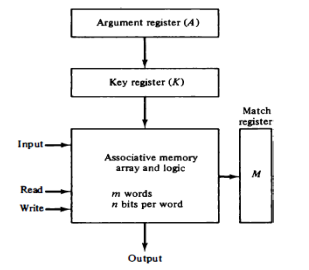
\includegraphics[width=0.7\linewidth]{associative}
    \caption{Associative memory circuit}\label{associative_circuit}
\end{figure}

\section{Neural associative memory}
Neural associative memory is also known as the associative network, which works
based on pattern association. It can store different patterns and produce the
output which closely matches the already given patterns. They are implemented
using the artificial neural network, which tries to mimic the working of the
brain. They are commonly used in applications like pattern recognition, data
storage and information retrieval. There are two types of associative networks
\begin{description}
    \item[Auto associative memory]A single layer NN in which the number of training
    vectors and the number of output vectors are the same. The weights are
    determined by the stored patterns
    \item[Hetero associative memory]A single layer NN in which the number of input
    training vectors and output are different. Weights are determined by the
    pattern stored in the network. It is static in nature and hence there would be
    no linear or delay operations
\end{description}

\subsection{Hopfield model}
The Hopfield model\cite{hopfield} is a type of RNN.\@ The model is designed to
mimic the behaviour of neurons in the brain. It is a type of associative memory
system and hence it can store and recall information based on the relationship
between the data stored. It has application including pattern recognition,
optimization, and error correction.

It is a fully connected NN and weights between connections determine the
strength of the connections. When the network is supplied with an input these
weights are updated sequentially until the network reaches a stable state, at
which the output is determined. By adjusting the weights in a specific way, the
the network is able to recall the information as a set of stable states

The main drawbacks of the model are that it may not converge to correct output
state when it is supplied with a pattern which is only partially similar to the
stored patterns or when it is not trained on sufficiently distinct data.

\section{\Snn}
Spiking neural networks are a type of neural network that models the behaviour
of biological neurons by using spikes or pulses to encode and transmit
information. They are a relatively new type of neural network that has the
potential to improve the performance and efficiency of artificial intelligence
systems. The use of spiking neural networks for building associative memory
systems is a relatively new area of research that has only recently started to
gain attention.
\subsection{Spike time dependent plasticity}
Spike-timing-dependent plasticity (STDP)\cite{stdp} is an unsupervised learning
rule based on the functioning of neurons in the brain for neuromorphic
computing, which is the study inspired by the structure and functioning of the
brain. In the process strength of the connection between neurons change based
on the relative timing of spikes or impulses

The basic idea behind STDP is that if two $N_{pre}$ and $N_{suc}$ neurons are
connected and their spike time are $t_1$ and $t_2$ respectively according to
STDP \vspace*{-.3pc}
\begin{itemize}
    \item[]Weight of connection from $N_{pre}$ to $N_{suc}$ should  increase, if {\boldmath$t_1>t_2$}
    \item[]Weight of connection from $N_{pre}$ to $N_{suc}$ should  decrease, if {\boldmath$t_1<t_2$}
    \item[]Weight of connection from $N_{pre}$ to $N_{suc}$ should  remain same, if {\boldmath$t_1=t_2$}
    \item[]
\end{itemize}
\vspace*{-2.5pc}
This process allows the neurons to adjust connection in a way which reflects
the relationship between input and output spikes signals.
\subsection{SpikeProp}
SpikeProp\cite{spikeprop} is an unsupervised learning algorithm used in the
field of neuromorphic computing used to train SNN based on the principle of
STDP.\@ It is similar to the gradient descent algorithm used in conventional deep
neural networks. It is computationally efficient and well-suited for real-time
applications. The issue with this algorithm is the need for a large amount of
data to achieve good results and only applicable to SNN.\@